\chapter{Field Failure Data Analysis}
	L'analisi di dati di fallimento è relativa ai log di errore dei sistemi \emph{Mercury} e \emph{BlueGene/L}. I dati erano già stati sottoposti alla fase di \emph{Filtering}. Si è potuto, quindi, procedere con la \emph{Manipulation}, utilizzando il metodo della \emph{Coalescenza temporale}, ed effettuare, infine, la \emph{Reliability Analysis}.\par
	Per determinare la finestra temporale è stata effettuata un'analisi di sensibilità del numero di tuple rispetto alla dimensione della finestra: sono state conteggiate le tuple al variare della finestra ed è stato trovato il valore ottimo di quest'ultima, alla destra del ginocchio della curva ottenuta. Per il sistema Mercury si è scelta una finestra temporale di $400s$, mentre per BlueGene di $200s$.
	\begin{figure}[H]
		\centering
		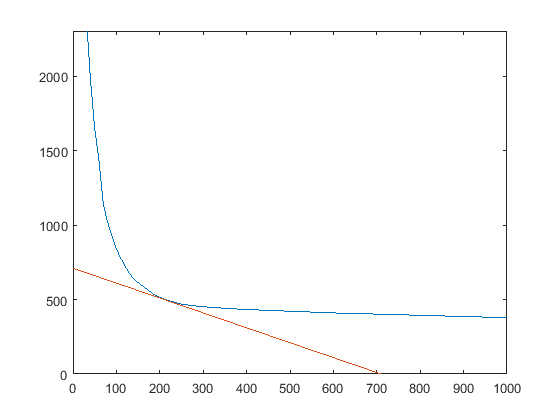
\includegraphics[scale=0.7]{./immagine/Mcwin.png}
		\caption{Sensitivity Analysis di Mercury}
		\label{fig:ffda-mcwin}
	\end{figure}
	\begin{figure}[H]
		\centering
		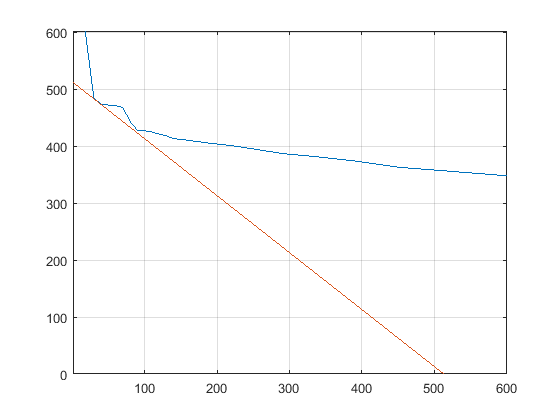
\includegraphics[scale=0.7]{./immagine/BGcwin.png}
		\caption{Sensitivity Analysis di BlueGene/L}
		\label{fig:ffda-bgcwin}
	\end{figure}
	Effettuanto il tupling, si ottengono 432 tuple per Mercury, 403 tuple per BlueGene. Sono presenti troncamenti e collisioni, che abbiamo provato ad individuare analizzando i file \emph{interarrivals} e \emph{lenghts}. Una tupla molto lunga può presentare collisioni al suo interno. Analogamente, tempi troppo brevi tra tuple possono essere un indizio di troncamento. In tal modo in Mercury si è individuato un troncamento tra le tuple 3 e 4, distanti $457s$, di un errore DEV nel nodo tg-c238, ed una collisione nella tupla 264 di errori dei nodi tg-c401 e tg-c027. In BlueGene osserviamo una collisione nella tupla 289 di errori di rack diversi.\par
	Mediante il file interarrivals, sono state calcolate le distribuzioni empiriche di TTF e Reliability dei due sistemi. Possiamo osservare come la curva della Reliability di BlueGene abbia un andamento più dolce, garantendo maggiore affidabilità.
	\begin{figure}[H]
		\centering
		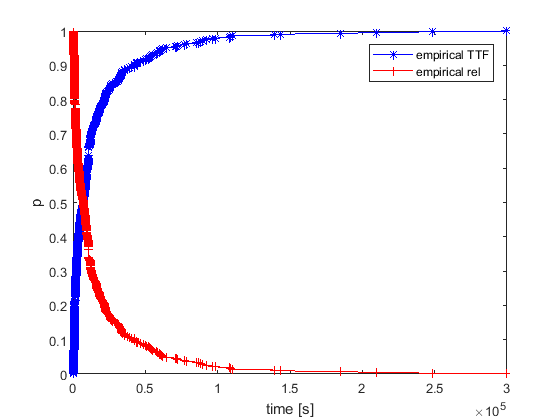
\includegraphics[scale=0.7]{./immagine/emprelM.png}
		\caption{Reliability empirica e TTF empirica di Mercury}
		\label{fig:ffda-emprelM}
	\end{figure}
	\begin{figure}[H]
		\centering
		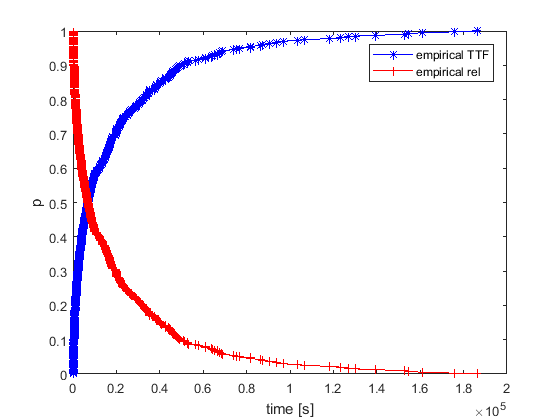
\includegraphics[scale=0.7]{./immagine/emprelBG.png}
		\caption{Reliability empirica e TTF empirica di BlueGene/L}
		\label{fig:ffda-emprelBG}
	\end{figure}
	Le curve empiriche sono state utilizzate per stimare i parametri delle distribuzioni teoriche. Sono state provate le distribuzioni esponenziale e di Weibull ed, in entrambi i casi, la seconda è risultata più aderente ai dati.
	\begin{figure}[H]
		\centering
		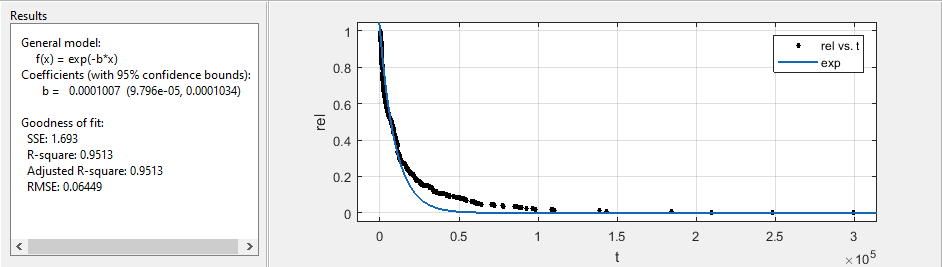
\includegraphics[scale=0.6]{./immagine/expM.png}
		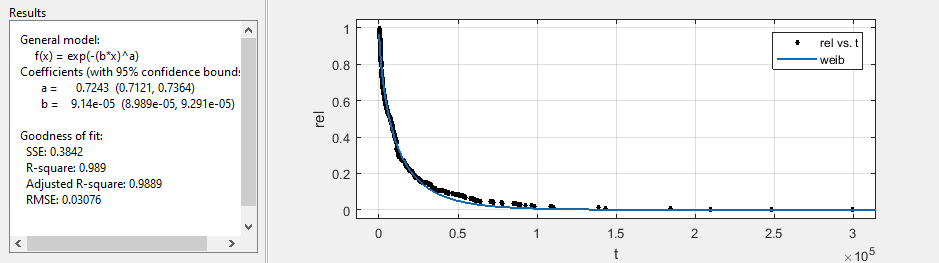
\includegraphics[scale=0.6]{./immagine/weibM.png}
		\caption{Fitting della Reliability empirica in Mercury}
		\label{fig:ffda-distrM}
	\end{figure}
	\begin{figure}[H]
		\centering
		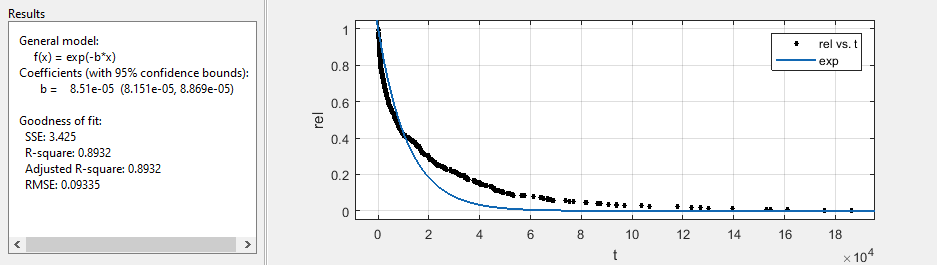
\includegraphics[scale=0.6]{./immagine/expBG.png}
		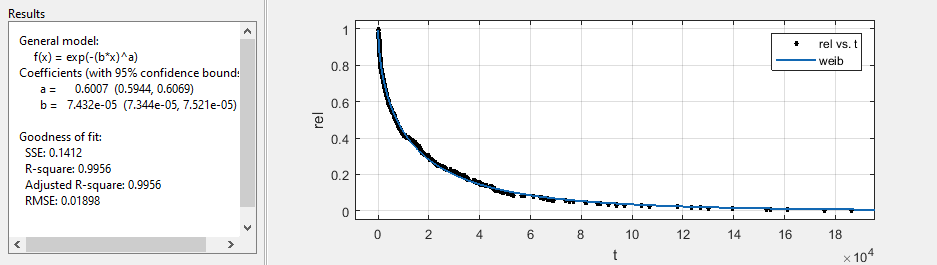
\includegraphics[scale=0.6]{./immagine/weibBG.png}
		\caption{Fitting della Reliability empirica in BlueGene}
		\label{fig:ffda-distrBG}
	\end{figure}
	La bontà del fitting è stata valutata con un test \emph{GOF}, in particolare il test di \emph{Kolmogorov-Smirnov} con livello di significatività pari a $0.05$. L'ipotesi che i dati seguano la distribuzione specifica è rigettata se $p<0.05$.
	\begin{table}
		\footnotesize
		\caption{Kolmogorov-Smirnov in Mercury}
		\label{tab:ffda-gofM}
		\centering
		\begin{tabular}{clcc}
			\toprule
			\textbf{Distribuzione} &
			\textbf{Ipotesi} &
			\textbf{P-value} &
			\textbf{K-statistic}\\
			\midrule
			Esponenziale &
			Rigettata &
			0.0081 &
			0.1152\\
			\midrule
			Weibull &
			Accettata &
			0.0657 &
			0.0907\\
			\bottomrule			
		\end{tabular}
	\end{table}
	\begin{table}
		\footnotesize
		\caption{Kolmogorov-Smirnov in BlueGene}
		\label{tab:ffda-gofBG}
		\centering
		\begin{tabular}{clcc}
			\toprule
			\textbf{Distribuzione} &
			\textbf{Ipotesi} &
			\textbf{P-value} &
			\textbf{K-statistic}\\
			\midrule
			Esponenziale &
			Rigettata &
			0.00060403 &
			0.1421\\
			\midrule
			Weibull &
			Accettata &
			0.2631 &
			0.0711\\
			\bottomrule			
		\end{tabular}
	\end{table}

	Assumendo, quindi, distribuzione di Weibull per entrambi i sistemi, possiamo calcolare MTTF (\textbf{Tabella \ref{tab:ffda-mttf}}).
	\begin{table}
		\footnotesize
		\caption{MTTF}
		\label{tab:ffda-mttf}
		\centering
		\begin{tabular}{clcc}
			\toprule
			\textbf{Sistema} &
			\textbf{MTTF [h]}\\
			\midrule
			Mercury &
			3.7281\\
			\midrule
			BlueGene/L &
			5.6154\\
			\bottomrule			
		\end{tabular}
	\end{table}
	
	
	\section{Analisi a livello di nodo}
		Prendiamo in analisi i primi 5 nodi con più occorrenze nei log dei due sistemi.
		Nel caso del sistema Mercury essi sono:
		\begin{itemize}
			\item \texttt{tg-c401} con 62340 occorrenze
			\item \texttt{tg-master} con 4098 occorrenze
			\item \texttt{tg-c572} con 4030 occorrenze
			\item \texttt{tg-s044} con 3224 occorrenze
			\item \texttt{tg-c238} con 1273 occorrenze
		\end{itemize}
		   Si filtrano i dati di log ad essi relativi per effettuare l'analisi di sensibilità e della reliability. Il procedimento è del tutto analogo a quello precedentemente seguito. Si riportano i risultati di seguito.
		
		\begin{figure}[H]
			\centering
			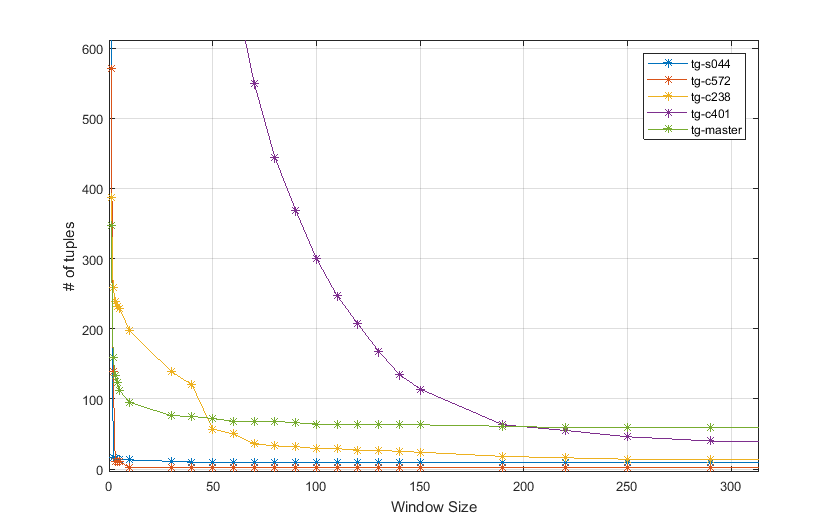
\includegraphics[scale=0.7]{./immagine/nodiMcwin.png}
			\caption{Sensitivity Analysis dei top-5 entries-prone nodes di Mercury}
			\label{fig:ffda-nMcwin}
		\end{figure}
	
		\begin{table}
			\footnotesize
			\caption{Coalescence Window dei top-5 entries-prone nodes di Mercury}
			\label{tab:ffda-nMcwin}
			\centering
			\begin{tabular}{clcc}
				\toprule
				\textbf{Nodo} &
				\textbf{Window Size [s]} &
				\textbf{Tuple Count}\\
				\midrule
				tg-c401 &
				300 &
				40\\
				\midrule
				tg-master &
				150 &
				63\\
				\midrule
				tg-c572 &
				10 &
				2\\
				\midrule
				tg-s044 &
				10 &
				13\\
				\midrule
				tg-c238 &
				150 &
				24\\
				\bottomrule			
			\end{tabular}
		\end{table}
		La dimensione delle finestre varia a seconda del nodo. Il nodo che funge da \emph{dependability-bottleneck} è tg-master, che ha ruolo di gestore nel sistema. Analizziamo i nodi con maggior numero di tuple.
		
		\begin{figure}[H]
			\centering
			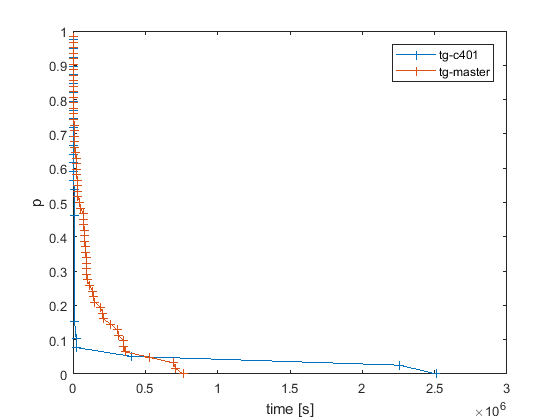
\includegraphics[scale=0.7]{./immagine/nodiMrel.png}
			\caption{Empirical Reliability degli entries-prone nodes di Mercury}
			\label{fig:ffda-nMrel}
		\end{figure}
		
		La Reliability di tg-master è superiore fino a $0.5*10^{6}s$, dopo il quale presenta una discesa molto più ripida di tg-c401, nodo di calcolo. Si ipotizza che il gestore debba avere una grande affidabilità, essendo un \emph{Single Point of Failure}, ma che sia soggetto ad una maggiore attenzione relativa alla manutenzione. Sembra quindi ragionevole che il tempo entro cui l'affidabilità è elevata sia il suo \emph{mission time}.\par
		
		Nel caso del sistema BlueGene/L i 5 nodi con più occorrenze nel log sono:
		\begin{itemize}
			\item \texttt{R71-M0-N4} con 1716 occorrenze
			\item \texttt{R12-M0-N0} con 1563 occorrenze
			\item \texttt{R63-M0-N2} con 976 occorrenze
			\item \texttt{R03-M1-NF} con 960 occorrenze
			\item \texttt{R63-M0-N0} con 791 occorrenze
		\end{itemize}
	
		\begin{figure}[H]
			\centering
			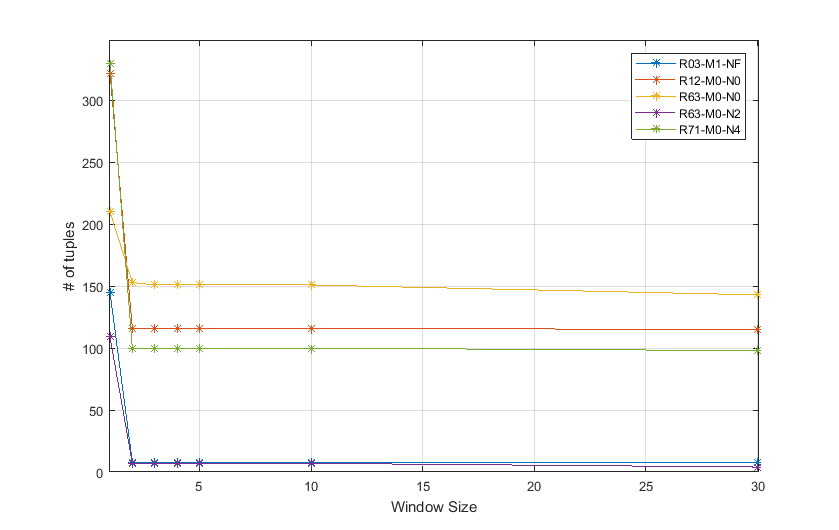
\includegraphics[scale=0.7]{./immagine/nodiBGcwin.png}
			\caption{Sensitivity Analysis dei top-5 entries-prone nodes di BlueGene/L}
			\label{fig:ffda-nBGcwin}
		\end{figure}
	
		\begin{table}
			\footnotesize
			\caption{Coalescence Window dei top-5 entries-prone nodes di BlueGene/l}
			\label{tab:ffda-nBGcwin}
			\centering
			\begin{tabular}{clcc}
				\toprule
				\textbf{Nodo} &
				\textbf{Window Size [s]} &
				\textbf{Tuple Count}\\
				\midrule
				R71-M0-N4 &
				10 &
				100\\
				\midrule
				R12-M0-N0 &
				10 &
				116\\
				\midrule
				R63-M0-N2 &
				10 &
				7\\
				\midrule
				R03-M1-NF &
				10 &
				8\\
				\midrule
				R63-M0-N0 &
				10 &
				151\\
				\bottomrule			
			\end{tabular}
		\end{table}
	
		In BlueGene la finestra temporale è la stessa per tutti i nodi (\textbf{Tabella \ref{tab:ffda-nBGcwin}}). Il numero di tuple, infatti, è molto sensibile fino ad una dimensione di circa $3s$ della finestra temporale, dopo la quale si stabilizza. Sono anche presenti dei \emph{dependability-bottleneck} con un grande numero di tuple: R71-M0-N4, R12-M0-N0, R63-M0-N0. Da notare che essi sono tutti nodi con la Compute Card di IO aggiuntiva. Presentano un andamento della Reliability simile, anche se risultano comunque essere più affidabili i rack con minori tuple (\textbf{Figura \ref{fig:ffda-nBGrel}}).
	
		\begin{figure}[H]
			\centering
			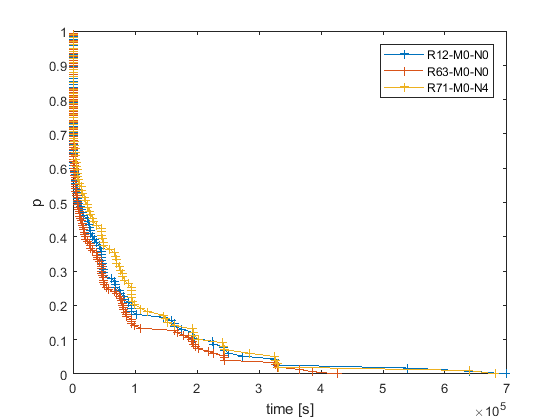
\includegraphics[scale=0.7]{./immagine/nodiBGrel.png}
			\caption{Empirical Reliability degli entries-prone nodes di BlueGene/L}
			\label{fig:ffda-nBGrel}
		\end{figure}
	
		\subsection{Nodi funzionalmente simili}
			Possiamo concentrarci su nodi con funzionalità simili.
			In Mercury tg-c401, tg-c572, tg-c238, tg-c242 sono tutti nodi di calcolo.  I primi tre sono stati analizzati anche precedentemente (\textbf{Tabella \ref{tab:ffda-nMcwin}}). L'ultimo nodo ha una finestra di $90s$ e conta 66 tuple. Essi hanno un numero di tuple ampiamente differente. Consideriamo, nello studio della Reliability, solo i nodi con più tuple. In \textbf{Figura \ref{fig:ffda-nCrel}} possiamo osservare come i nodi di calcolo presentino un andamento della Reliability comune, che tende prima ad abbattersi velocemente, per poi tendere lentamente a 0.
			
			\begin{figure}[H]
				\centering
				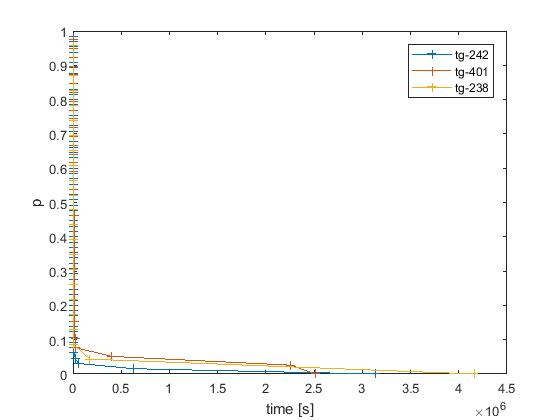
\includegraphics[scale=0.6]{./immagine/nodiCrel.jpg}
				\caption{Empirical Reliability dei nodi di calcolo di Mercury}
				\label{fig:ffda-nCrel}
			\end{figure}
			
			In BlueGene/L sono nodi funzionalmente simili R71-M0-N4, R12-M0-N0, R63-M0-N0, poiché tutti di IO. Essi, come già osservato, presentano tutti un grande numero di tuple con la stessa finestra temporale (\textbf{Tabella \ref{tab:ffda-nBGcwin}}). Anche la relativa Reliability presenta un andamento simile (\textbf{Figura \ref{fig:ffda-nBGrel}}).
	
	\section{Analisi a livello di errore}
		Possiamo procedere allo stesso modo per le categorie di errore dei nodi di Mercury e le Compute Unit di BlueGene/L.\par
		In Mercury le categorie di errore più frequenti sono:
		\begin{itemize}
			\item \textbf{DEV}
			\item \textbf{MEM}
			\item \textbf{IO}
			\item \textbf{NET}
			\item \textbf{PRO}
		\end{itemize}
		
		\begin{figure}[H]
			\centering
			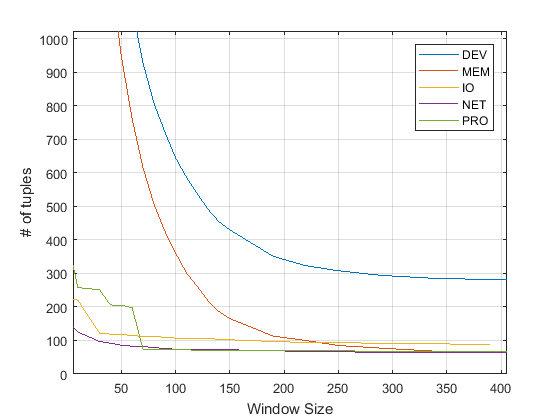
\includegraphics[scale=0.7]{./immagine/categorieMcwin.png}
			\caption{Sensitivity Analysis delle categorie di errore di Mercury}
			\label{fig:ffda-cMcwin}
		\end{figure}
		Gli errori con più tuple sono relativi all'interconnessione ed alle operazioni di IO. 
	
		\begin{table}
			\footnotesize
			\caption{Coalescence Window delle categorie di errore di Mercury}
			\label{tab:ffda-cMcwin}
			\centering
			\begin{tabular}{clcc}
				\toprule
				\textbf{Errore} &
				\textbf{Window Size [s]} &
				\textbf{Tuple Count}\\
				\midrule
				DEV &
				350 &
				284\\
				\midrule
				MEM &
				350 &
				68\\
				\midrule
				IO &
				70 &
				112\\
				\midrule
				NET &
				80 &
				79\\
				\midrule
				PRO &
				100 &
				73\\
				\bottomrule			
			\end{tabular}
		\end{table}
		
		\begin{figure}[H]
			\centering
			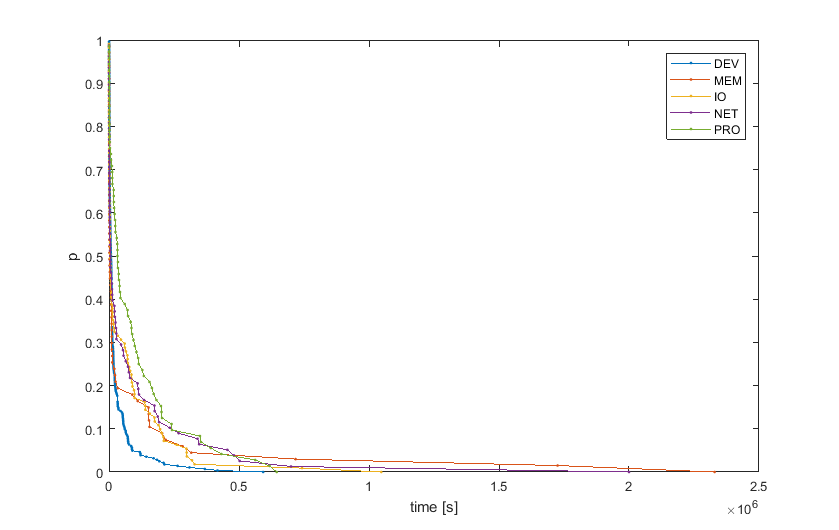
\includegraphics[scale=0.7]{./immagine/categorieMrel.png}
			\caption{Empirical Reliability delle categorie di errore di Mercury}
			\label{fig:ffda-cMrel}
		\end{figure}
	
		L'interconnessione risulta essere una risorsa critica con una Reliability che si abbatte più velocemente delle altre.\par
		Si analizzano le Compute Unit relative all'IO di BlueGene/L:
		\begin{itemize}
			\item \texttt{J18-U11}
			\item \texttt{J18-U01}
		\end{itemize}
		
		Entrambe le unità hanno un alto numero di tuple e la stessa dimensione per la finestra temporale. Il numero di tuple presenta, infatti, andamento simile, al variare della dimensione della finestra. Ciò è comprensibile anche alla luce del fatto che sono entrambe unità facenti parte di Compute Card di IO.
		
		\begin{figure}[H]
			\centering
			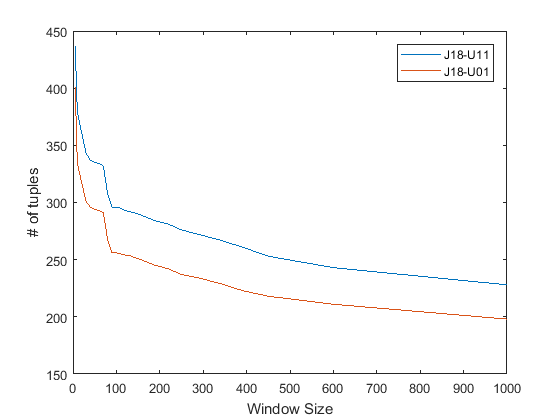
\includegraphics[scale=0.7]{./immagine/categorieBGcwin.png}
			\caption{Sensitivity Analysis delle Compute Unit di BlueGene/L}
			\label{fig:ffda-cBGcwin}
		\end{figure}
	
		\begin{table}
			\footnotesize
			\caption{Coalescence Window delle Compute Unit di BlueGene/L}
			\label{tab:ffda-cBGcwin}
			\centering
			\begin{tabular}{clcc}
				\toprule
				\textbf{Compute Unit} &
				\textbf{Window Size [s]} &
				\textbf{Tuple Count}\\
				\midrule
				J18-U11 &
				100 &
				296\\
				\midrule
				J18-U01 &
				100 &
				256\\
				\bottomrule			
			\end{tabular}
		\end{table}
	
		\begin{figure}[H]
			\centering
			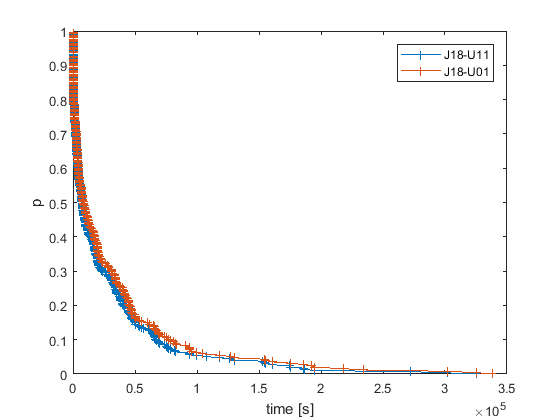
\includegraphics[scale=0.7]{./immagine/categorieBGrel.png}
			\caption{Empirical Reliability delle Compute Unit di BlueGene/L}
			\label{fig:ffda-cBGrel}
		\end{figure}
	
		Analoga è anche la curva della Reliability, comunque leggermente superiore per l'unità U01 con meno tuple.
		
	\section{Analisi combinata}
		In Mercury estraiamo i 5 nodi più ricorrenti dai log di ogni categoria di errore.
		\begin{table}
			\footnotesize
			\caption{Nodi più ricorrenti per categoria di errore in Mercury}
			\label{tab:ffda-Minn}
			\centering
			\begin{tabular}{clllll}
				\toprule
				\textbf{} &
				\textbf{DEV} &
				\textbf{MEM} &
				\textbf{IO} &
				\textbf{NET} &
				\textbf{PRO}\\
				\midrule
				1 &
				tg-c401 50782 &
				tg-c401 11558 &
				tg-s044 3208 &
				tg-master 3639 &
				tg-c648 616\\
				\midrule
				2 &
				tg-c572 3176 &
				tg-c572 845 &
				tg-master 452 &
				tg-c550 33 &
				tg-c324 239\\
				\midrule
				3 &
				tg-c238 1071 &
				tg-c238 197 &
				tg-login3 381 &
				tg-c196 14 &
				tg-c284 180\\
				\midrule
				4 &
				tg-c242 918 &
				tg-c242 149 &
				tg-s038 230 &
				tg-c238 3 &
				tg-c451 159\\
				\midrule
				5 &
				tg-c117 263 &
				tg-c894 28 &
				tg-c550 220 &
				tg-s044 2 &
				tg-c447 136\\
				\bottomrule			
			\end{tabular}
		\end{table}
		In \textbf{Tabella \ref{tab:ffda-Minn}} possiamo notare come i nodi di calcolo siano la causa esclusiva di errori di tipo DEV, MEM e PRO. In particolare, i nodi fonte di errori DEV e MEM sono gli stessi, il che può far sospettare ad una comunanza di fault. Come ci si poteva aspettare, gli errori di IO sono causati principalmente da nodi di storage, di login e dal master. Infine gli errori NET di rete sono quasi totalmente ascrivibili al nodo master.\par
		In BlueGene/L siamo interessati ai rack con maggior numero di occorrenze nel log. Per fare ciò sono state omesse le informazioni sul midplane e sul nodo.
		\begin{table}
			\footnotesize
			\caption{Rack con maggiori eventi di errore di BlueGene/L}
			\label{tab:ffda-BGr}
			\centering
			\begin{tabular}{clcc}
				\toprule
				\textbf{} &
				\textbf{Rack} &
				\textbf{Occorrenze}\\
				\midrule
				1 &
				R63 &
				7192\\
				\midrule
				2 &
				R62 &
				4057\\
				\midrule
				3 &
				R57 &
				3581\\
				\midrule
				4 &
				R56 &
				3527\\
				\midrule
				5 &
				R46 &
				3485\\
				\bottomrule			
			\end{tabular}
		\end{table}
		In \textbf{Tabella \ref{tab:ffda-BGr}} osserviamo che il rack con più eventi di errore è R63. Precedentemente abbiamo riscontrato che i nodi N0 e N2 di questo rack fanno anche parte della top-5 entries-prone nodes. I rack che abbiamo trovato sono tutti vicini tra loro. Sembra ragionevole, nel calcolo scientifico, parallelizzare i calcoli, assegnandoli a nodi vicini, fino a coinvolgere interi rack. Può essere plausibile, dunque, una relazione tra l'elevato numero di eventi di errore che essi presentano.